\chapter{Thực hiện các thuật toán tìm kiếm}

\section{BFS}

\begin{figure}[H]
    \centering
    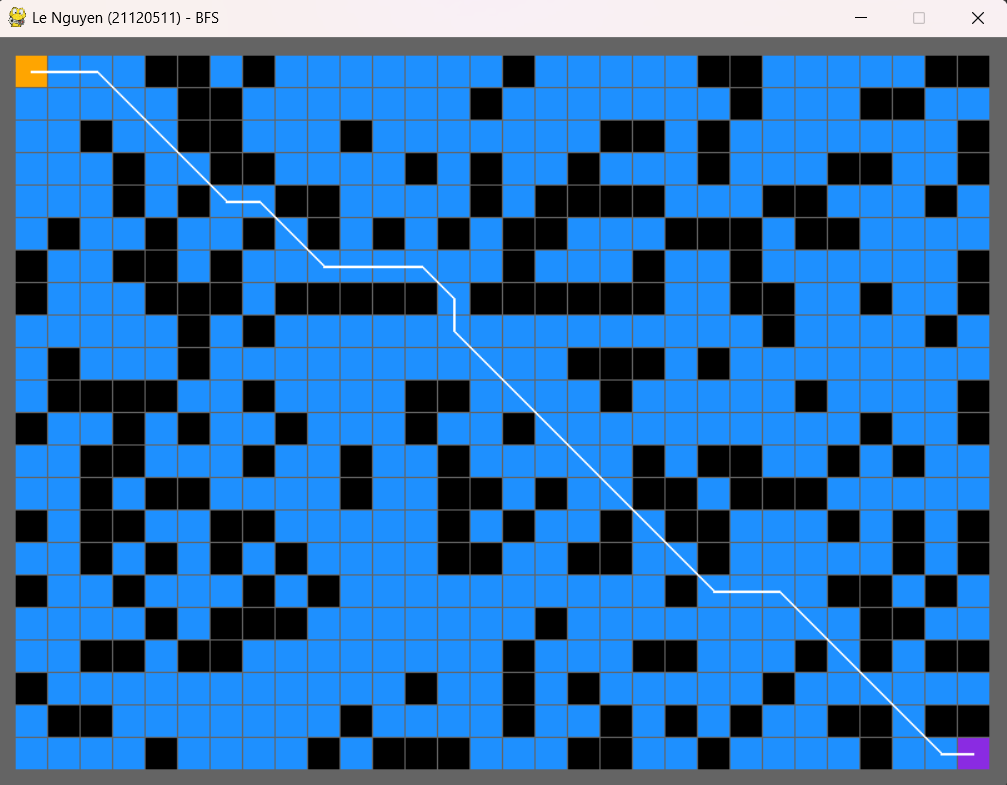
\includegraphics[scale=0.7]{figure/Implementation/BFS.png}
    \caption{BFS được thực hiện trên một mê cung.}
    \label{fig:imple_BFS}
\end{figure}

Ta có thể thấy BFS đã tìm kiếm hết toàn bộ các ô trong mê cung, (các ô nằm trong $expanded$ sẽ được tô màu xanh). Trong quá trình tìm kiếm BFS sẽ cố gắng mở rộng theo chiều rộng các nút với thứ tự [up, down, left, right, left\_up, left\_down, right\_up, right\_down].

\section{UCS}

\begin{figure}[H]
    \centering
    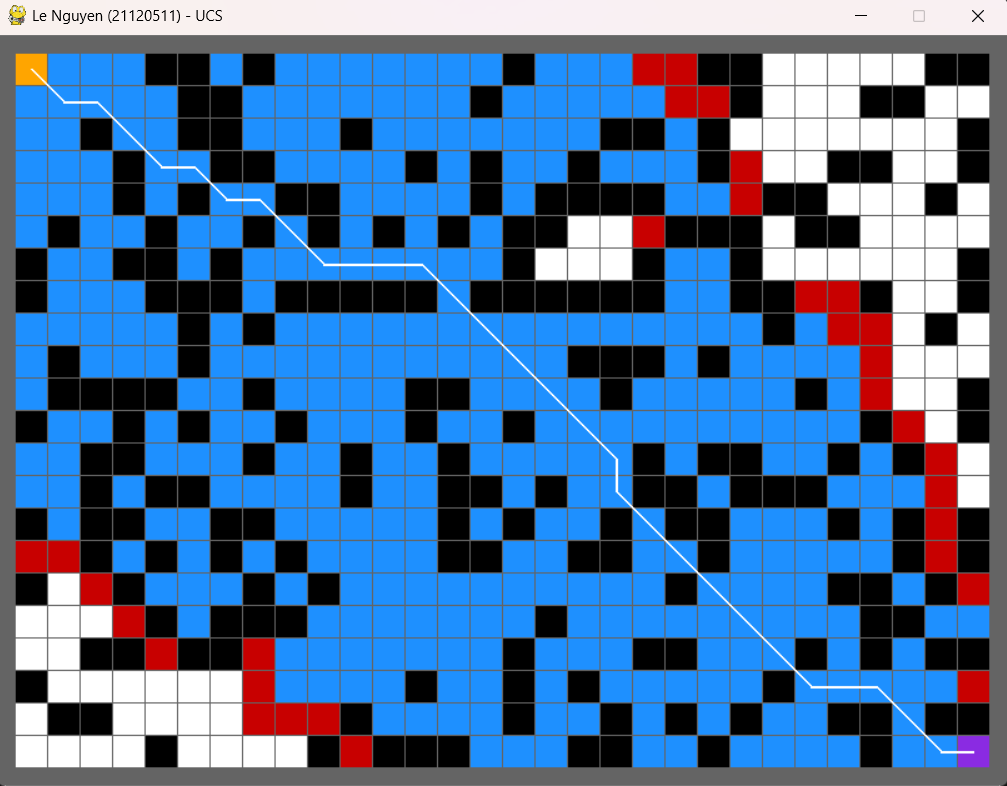
\includegraphics[scale=0.7]{figure/Implementation/UCS.png}
    \caption{UCS được thực hiện trên một mê cung}
    \label{fig:imple_UCS}
\end{figure}

Ở UCS, ta sẽ xét trọng số mỗi node theo chính thứ tự của nó như sau: [up = 6, down = 3, left = 7, right = 2, left\_up = 8, left\_down = 5, right\_up = 4, right\_down = 1]. Khi đó UCS của ta sẽ ưu tiên đi hướng xuống nghiêng về phía bên phải, vì vậy như hình phía trên các nút được mở rộng (màu xanh) có xu hướng tập trung về phía xuống nghiêng bên phải của mê cung.

\section{DFS}

\begin{figure}[H]
    \centering
    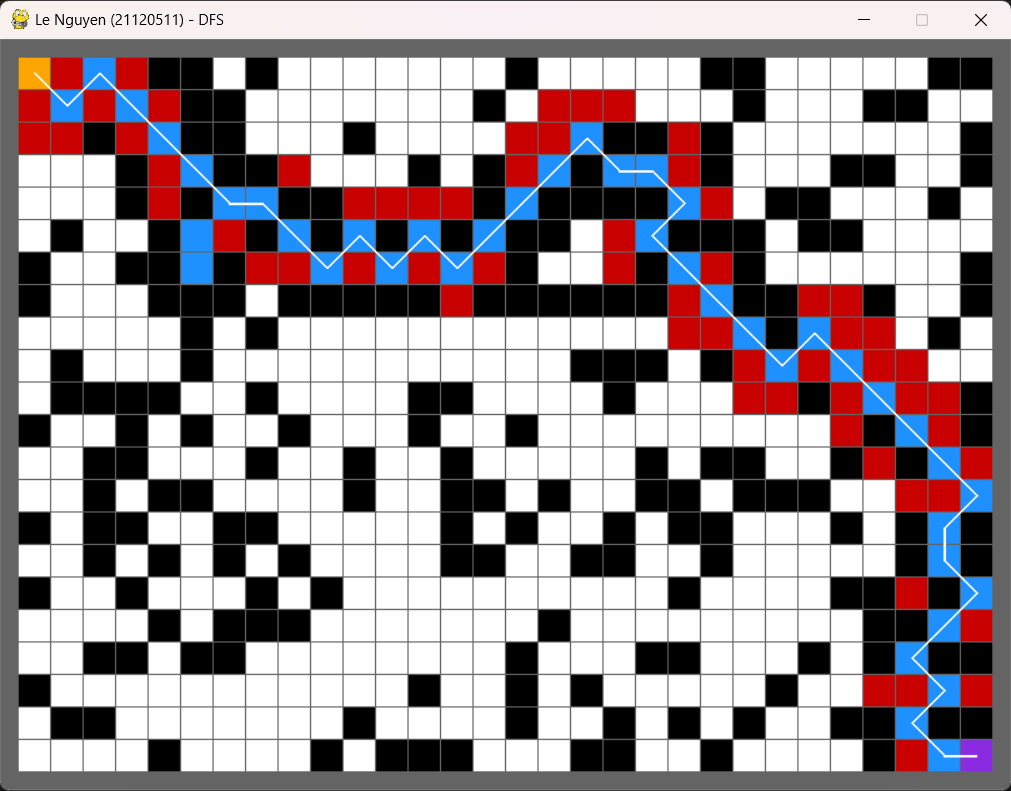
\includegraphics[scale=0.7]{figure/Implementation/DFS.png}
    \caption{DFS được thực hiện trên một mê cung}
    \label{fig:imple_DFS}
\end{figure}

So các nút được thêm vào theo thứ tự [up, down, left, right, left\_up, left\_down, right\_up, right\_down] nên theo cơ chế ngăn xếp của DFS, những nút right\_down sẽ được lấy ra trước và ta có một kết quả như trên.

\section{$\text{A}^*$}

\begin{figure}[H]
    \centering
    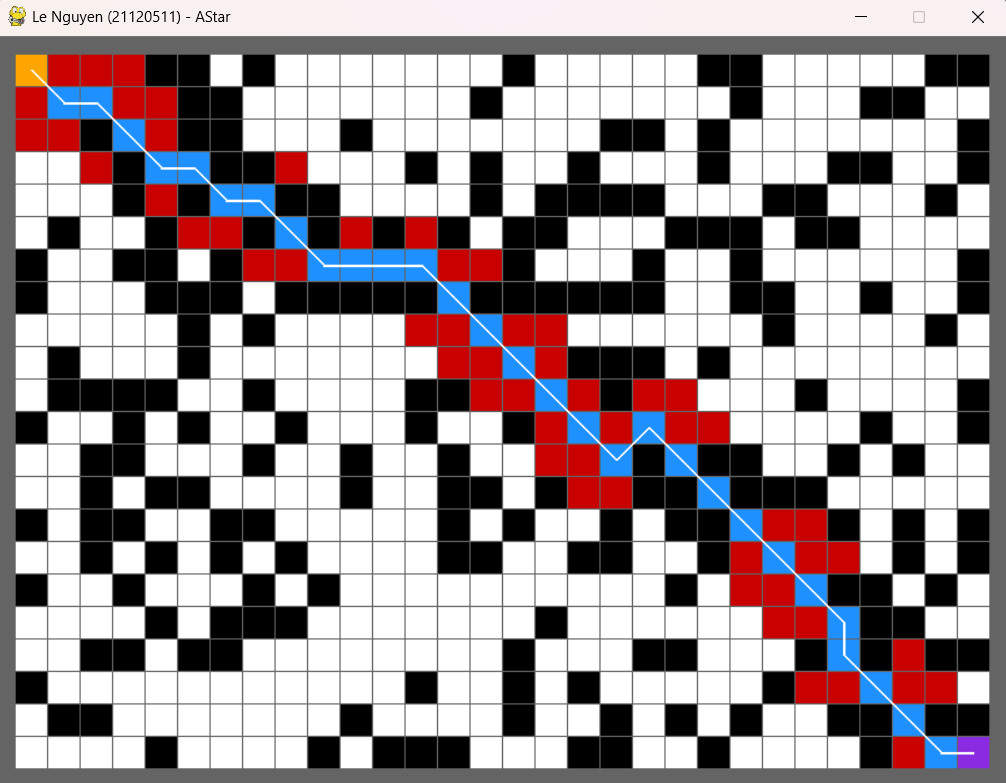
\includegraphics[scale=0.7]{figure/Implementation/AStar.png}
    \caption{$\text{A}^{*}$ được thực hiện trên một mê cung}
    \label{fig:imple_AStar}
\end{figure}

Như ta đã nói phía trên, ta sẽ chọn hàm $heuristic$ là \textit{chebyshev distance} do bài toán được thực hiện trên một mặt phẳng hai chiều, chia thành các ô vuông. Ở \textit{chebyshev distance} thuật toán của ta sẽ tối ưu hơn cho 8 hướng (thay vì 4 hướng như \textit{manhattan distance}, \textit{mahattan distance} không thể đi xéo được). Kết hợp thêm trọng số được đặt như UCS, $\text{A}^*$ của ta sẽ đi một mạch hướng xuống nghiêng bên phải để đi về đích, dựa trên hình, ta cũng có thể thấy $\text{A}^*$ nhanh và cũng tốn ít bộ nhớ nhất (số nút ô màu ít hơn).

\section{Greedy}

\begin{figure}[H]
    \centering
    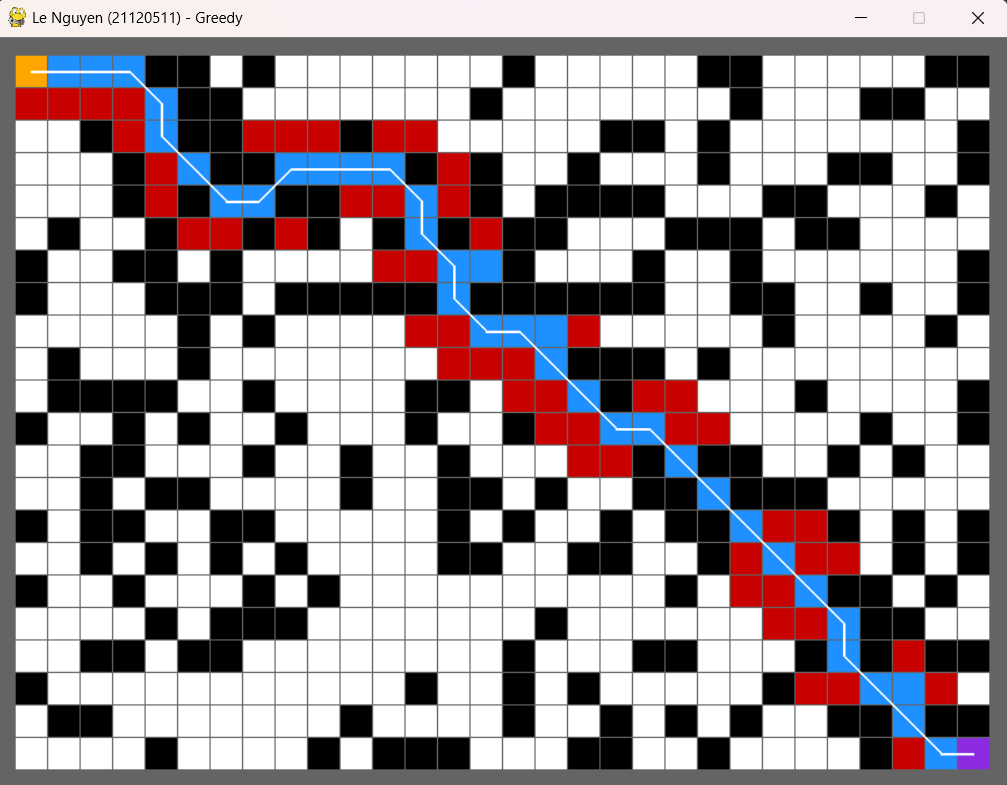
\includegraphics[scale=0.7]{figure/Implementation/Greedy.png}
    \caption{Greedy được thực hiện trên một mê cung}
    \label{fig:imple_Greedy}
\end{figure}

Ở Greedy ta cũng dùng hàm heuristic là \textit{chebyshev distance} như $A^*$ nên Greedy cũng có xu hướng đi xuống nghiêng về bên phải, ta thấy Greedy có đường đi dài hơn $\text{A}^*$ do nó chỉ quan tâm đến heuristic mà bỏ quên đi chi phí đường đi.